% Options for packages loaded elsewhere
\PassOptionsToPackage{unicode}{hyperref}
\PassOptionsToPackage{hyphens}{url}
%
\documentclass[
  man,floatsintext]{apa6}
\usepackage{amsmath,amssymb}
\usepackage{lmodern}
\usepackage{iftex}
\ifPDFTeX
  \usepackage[T1]{fontenc}
  \usepackage[utf8]{inputenc}
  \usepackage{textcomp} % provide euro and other symbols
\else % if luatex or xetex
  \usepackage{unicode-math}
  \defaultfontfeatures{Scale=MatchLowercase}
  \defaultfontfeatures[\rmfamily]{Ligatures=TeX,Scale=1}
\fi
% Use upquote if available, for straight quotes in verbatim environments
\IfFileExists{upquote.sty}{\usepackage{upquote}}{}
\IfFileExists{microtype.sty}{% use microtype if available
  \usepackage[]{microtype}
  \UseMicrotypeSet[protrusion]{basicmath} % disable protrusion for tt fonts
}{}
\makeatletter
\@ifundefined{KOMAClassName}{% if non-KOMA class
  \IfFileExists{parskip.sty}{%
    \usepackage{parskip}
  }{% else
    \setlength{\parindent}{0pt}
    \setlength{\parskip}{6pt plus 2pt minus 1pt}}
}{% if KOMA class
  \KOMAoptions{parskip=half}}
\makeatother
\usepackage{xcolor}
\usepackage{graphicx}
\makeatletter
\def\maxwidth{\ifdim\Gin@nat@width>\linewidth\linewidth\else\Gin@nat@width\fi}
\def\maxheight{\ifdim\Gin@nat@height>\textheight\textheight\else\Gin@nat@height\fi}
\makeatother
% Scale images if necessary, so that they will not overflow the page
% margins by default, and it is still possible to overwrite the defaults
% using explicit options in \includegraphics[width, height, ...]{}
\setkeys{Gin}{width=\maxwidth,height=\maxheight,keepaspectratio}
% Set default figure placement to htbp
\makeatletter
\def\fps@figure{htbp}
\makeatother
\setlength{\emergencystretch}{3em} % prevent overfull lines
\providecommand{\tightlist}{%
  \setlength{\itemsep}{0pt}\setlength{\parskip}{0pt}}
\setcounter{secnumdepth}{-\maxdimen} % remove section numbering
% Make \paragraph and \subparagraph free-standing
\ifx\paragraph\undefined\else
  \let\oldparagraph\paragraph
  \renewcommand{\paragraph}[1]{\oldparagraph{#1}\mbox{}}
\fi
\ifx\subparagraph\undefined\else
  \let\oldsubparagraph\subparagraph
  \renewcommand{\subparagraph}[1]{\oldsubparagraph{#1}\mbox{}}
\fi
\newlength{\cslhangindent}
\setlength{\cslhangindent}{1.5em}
\newlength{\csllabelwidth}
\setlength{\csllabelwidth}{3em}
\newlength{\cslentryspacingunit} % times entry-spacing
\setlength{\cslentryspacingunit}{\parskip}
\newenvironment{CSLReferences}[2] % #1 hanging-ident, #2 entry spacing
 {% don't indent paragraphs
  \setlength{\parindent}{0pt}
  % turn on hanging indent if param 1 is 1
  \ifodd #1
  \let\oldpar\par
  \def\par{\hangindent=\cslhangindent\oldpar}
  \fi
  % set entry spacing
  \setlength{\parskip}{#2\cslentryspacingunit}
 }%
 {}
\usepackage{calc}
\newcommand{\CSLBlock}[1]{#1\hfill\break}
\newcommand{\CSLLeftMargin}[1]{\parbox[t]{\csllabelwidth}{#1}}
\newcommand{\CSLRightInline}[1]{\parbox[t]{\linewidth - \csllabelwidth}{#1}\break}
\newcommand{\CSLIndent}[1]{\hspace{\cslhangindent}#1}
\ifLuaTeX
\usepackage[bidi=basic]{babel}
\else
\usepackage[bidi=default]{babel}
\fi
\babelprovide[main,import]{english}
% get rid of language-specific shorthands (see #6817):
\let\LanguageShortHands\languageshorthands
\def\languageshorthands#1{}
% Manuscript styling
\usepackage{upgreek}
\captionsetup{font=singlespacing,justification=justified}

% Table formatting
\usepackage{longtable}
\usepackage{lscape}
% \usepackage[counterclockwise]{rotating}   % Landscape page setup for large tables
\usepackage{multirow}		% Table styling
\usepackage{tabularx}		% Control Column width
\usepackage[flushleft]{threeparttable}	% Allows for three part tables with a specified notes section
\usepackage{threeparttablex}            % Lets threeparttable work with longtable

% Create new environments so endfloat can handle them
% \newenvironment{ltable}
%   {\begin{landscape}\begin{center}\begin{threeparttable}}
%   {\end{threeparttable}\end{center}\end{landscape}}
\newenvironment{lltable}{\begin{landscape}\begin{center}\begin{ThreePartTable}}{\end{ThreePartTable}\end{center}\end{landscape}}

% Enables adjusting longtable caption width to table width
% Solution found at http://golatex.de/longtable-mit-caption-so-breit-wie-die-tabelle-t15767.html
\makeatletter
\newcommand\LastLTentrywidth{1em}
\newlength\longtablewidth
\setlength{\longtablewidth}{1in}
\newcommand{\getlongtablewidth}{\begingroup \ifcsname LT@\roman{LT@tables}\endcsname \global\longtablewidth=0pt \renewcommand{\LT@entry}[2]{\global\advance\longtablewidth by ##2\relax\gdef\LastLTentrywidth{##2}}\@nameuse{LT@\roman{LT@tables}} \fi \endgroup}

% \setlength{\parindent}{0.5in}
% \setlength{\parskip}{0pt plus 0pt minus 0pt}

% Overwrite redefinition of paragraph and subparagraph by the default LaTeX template
% See https://github.com/crsh/papaja/issues/292
\makeatletter
\renewcommand{\paragraph}{\@startsection{paragraph}{4}{\parindent}%
  {0\baselineskip \@plus 0.2ex \@minus 0.2ex}%
  {-1em}%
  {\normalfont\normalsize\bfseries\itshape\typesectitle}}

\renewcommand{\subparagraph}[1]{\@startsection{subparagraph}{5}{1em}%
  {0\baselineskip \@plus 0.2ex \@minus 0.2ex}%
  {-\z@\relax}%
  {\normalfont\normalsize\itshape\hspace{\parindent}{#1}\textit{\addperi}}{\relax}}
\makeatother

% \usepackage{etoolbox}
\makeatletter
\patchcmd{\HyOrg@maketitle}
  {\section{\normalfont\normalsize\abstractname}}
  {\section*{\normalfont\normalsize\abstractname}}
  {}{\typeout{Failed to patch abstract.}}
\patchcmd{\HyOrg@maketitle}
  {\section{\protect\normalfont{\@title}}}
  {\section*{\protect\normalfont{\@title}}}
  {}{\typeout{Failed to patch title.}}
\makeatother

\usepackage{xpatch}
\makeatletter
\xapptocmd\appendix
  {\xapptocmd\section
    {\addcontentsline{toc}{section}{\appendixname\ifoneappendix\else~\theappendix\fi\\: #1}}
    {}{\InnerPatchFailed}%
  }
{}{\PatchFailed}
\keywords{teaching, intention, skill transmission, musical expression}
\usepackage{csquotes}
\ifLuaTeX
  \usepackage{selnolig}  % disable illegal ligatures
\fi
\IfFileExists{bookmark.sty}{\usepackage{bookmark}}{\usepackage{hyperref}}
\IfFileExists{xurl.sty}{\usepackage{xurl}}{} % add URL line breaks if available
\urlstyle{same} % disable monospaced font for URLs
\hypersetup{
  pdftitle={What makes musicians infer teaching intentions?},
  pdfauthor={Atsuko Tominaga1,*, Günther Knoblich1, \& Natalie Sebanz1},
  pdflang={en-EN},
  pdfkeywords={teaching, intention, skill transmission, musical expression},
  hidelinks,
  pdfcreator={LaTeX via pandoc}}

\title{What makes musicians infer teaching intentions?}
\author{Atsuko Tominaga\textsuperscript{1,*}, Günther Knoblich\textsuperscript{1}, \& Natalie Sebanz\textsuperscript{1}}
\date{}


\shorttitle{What makes musicians infer teaching intentions?}

\affiliation{\vspace{0.5cm}\textsuperscript{1} Department of Cognitive Science, Central European University, Quellenstraße 51, 1100 Vienna, Austria\\\textsuperscript{*} Corresponding author: \href{mailto:Tominaga_Atsuko@phd.ceu.edu}{\nolinkurl{Tominaga\_Atsuko@phd.ceu.edu}}}

\abstract{
Perceiving pedagogical intentions is vital when learning skills from others. Our previous research demonstrated that expert pianists systematically modulated their sound so as to teach musical expressive techniques such as articulation and dynamics. For example, pianists played slower and exaggerated each technique when they had an intention to teach. Here we investigated whether the modulations that expert pianists produce when they intend to teach are also perceived by listeners as conveying pedagogical intentions. In the current study, musicians listened to piano recordings where a musical expressive technique of either articulation or dynamics was implemented. Half of the recordings was produced when pianists were instructed to play as if they were teaching the designated musical technique in a lesson (i.e., teaching recordings) whereas the other half was produced when pianists were instructed to play as if they were performing it in a concert (i.e., performing recordings). Participants were asked to judge whether each recording was produced for teaching purposes or not. We calculated the accuracy of participants' judgments to investigate whether they could distinguish teaching recordings from performing recordings. Also, recordings were quantified with regard to tempo, articulation and dynamic so that we could perform correlation and multiple regression analysis to investigate which features of piano performance made musicians infer teaching intentions. The findings in Experiment 1 with a simple musical scale demonstrated that the accuracy of musicians' judgments was significantly above chance. Also, it was found that slower tempo contributed to musicians' judgments as teaching regardless of the techniques. Moreover, performances with exaggeration for each technique (e.g., longer legato, shorter staccato, larger contrast between forte and piano) were more likely to be judged as teaching. Experiment 2 aimed to replicate the findings of Experiment 1 with a more naturalistic piece. As Experiment 1, the accuracy of musicians' judgments was significantly above chance. However, we only replicated that performances with exaggerated dynamics (in particular, larger contrast between forte and piano) were more likely to be judged as teaching. Taken together, loudness (dynamics) seems to be reliably used to infer teaching intentions regardless of the complexity of a musical piece. Also, typical pedagogical behaviour such as slowing down may not be necessarily perceived as teaching performance when learning complex skills such as artistic expression.
}



\begin{document}
\maketitle

\hypertarget{introduction}{%
\section{Introduction}\label{introduction}}

Learning from others is one of the important elements of skill acquisition. Not only are we able to learn by observing and imitating others, but also we benefit greatly from interacting with others such as teachers and peers (Tomasello, Kruger, \& Ratner, 1993). Adults are often being pedagogical to children in order to explain and transmit cultural conventions (Csibra \& Gergely, 2009). Active teaching seems to play a crucial role not only to transit skills over generations but also to further develop sophisticated cultures, which cannot be achieved by one single individual or generation (Tennie, Call, \& Tomasello, 2009). From a learner's perspective, it is important to identify informative teachers and infer teachers' expectations so that learners can acquire skills through interacting with teachers (Gweon, 2020; Veissière, Constant, Ramstead, Friston, \& Kirmayer, 2020).

In pedagogical settings where teachers are supposed to convey useful information to learners, it has been found that teachers often modulate their behaviour for teaching purposes. For example, adults are likely to modulate their speech and action for infants so as to help infants acquire skills (e.g., Brand, Baldwin, \& Ashburn, 2002; Saint-Georges et al., 2013). Further studies have revealed that even towards adult learners, people modulated their speech and action in a similar way as they did for infants (McEllin, Knoblich, \& Sebanz, 2017; Uther, Knoll, \& Burnham, 2007). Moreover, McEllin, Sebanz, and Knoblich (2018) demonstrated that people could identify informative intentions such as acting with others or teaching by relying on specific kinematics cues (e.g., velocity profiles of movements). These findings suggest that experts modified their speech and action to send teaching intentions and that novices could successfully perceive the intentions.

Tominaga, Knoblich \& Sebanz (\emph{submitted}) extended this line of research to expertise transmission where skills to be acquired are complex, such as when learning to perform with artistic expression. We investigated whether and how expert pianists are able to communicatively modulate their performance when intending to teach the musical expressive techniques of articulation (the smoothness of sound) and dynamics (the loudness of sound). The results demonstrated that expert pianists systematically modulated their performance by playing slower or by exaggerating relevant aspects of the performance (e.g., producing shorter staccato or producing a larger contrast between forte and piano) when intending to teach the musical expressive techniques. Therefore, it seems that even in the domain of expertise, experts exhibit pedagogical behaviours to highlight crucial performance aspects for potential learners.

Here we investigated whether the modulations that expert pianists make when they intended to teach are also perceived by listeners as conveying teaching intentions. We started from the assumption that listeners would be able to infer intentions from listening to recordings because previous research revealed that sound alone is sufficient to communicate different aspects of a musical performance. For instance, listeners are well able to infer performers' intended emotions when listening to recorded performances (e.g., Akkermans et al., 2019; Gabrielsson \& Juslin, 1996).

In the present study, musicians listened to piano recordings where a musical expressive technique of either articulation or dynamics was implemented. They were asked to judge whether each recording was produced for teaching purposes or not. Half of the recordings was produced when pianists were instructed to play as if they were teaching the designated musical technique in a lesson (i.e., teaching recordings) whereas the other half was produced when pianists were instructed to play as if they were performing it in a concert (i.e., performing recordings). First, we calculated the accuracy of participants' judgments to examine whether they could distinguish teaching recordings from performing recordings. Furthermore, recordings were quantified with regard to tempo, articulation and dynamic. Using correlations and multiple regression analysis, we examined which modulations of performance were used to infer teaching intentions.

If performers' intentions are understood by learners with basic musical skills, listeners should be able to distinguish teaching recordings from performing recordings. Moreover, the same modulations of pedagogical performance parameters observed in our previous experiments such as slower demonstration and exaggerated performance, should be used to infer teaching intentions by the earners. In Experiment 1 learners listened to performances with that followed simple musical scales. In Experiment 2 learners listen to performances of a more naturalistic piece of music in aan attempt to replicate the findings from Experiment 1.

\hypertarget{experiment-1}{%
\section{Experiment 1}\label{experiment-1}}

\hypertarget{methods}{%
\section{Methods}\label{methods}}

\hypertarget{participants}{%
\subsection{Participants}\label{participants}}

We recruited 21 participants who had at least six years of training in any musical instrument. They were able to read sheet music and knew two musical expressive techniques of articulation and dynamics. One participant was excluded due to an experimental error. Therefore, 20 participants (Female: 13) were included for data analysis and had 11.8 years of musical training on average (\emph{SD} = 5.62). They were all right-handed with a mean age of 28.8 (\emph{SD} = 9.09). All participants were recruited through an online participant platform (SONA system, \url{https://www.sona-systems.com}). The study (No.~2020/02) was approved by the Psychological Research Ethics Board (PREBO) CEU PU in Austria.

\hypertarget{apparatus}{%
\subsection{Apparatus}\label{apparatus}}

The experiment was programmed in Python 3.8.2 using the PsychoPy Python library (2020.2.4; \url{https://www.psychopy.org/}) on a Mac Book Pro with Mac OS X Catalina 10.15.6. Stimuli were played using the Mido Python library (1.2.9; \url{https://mido.readthedocs.io/en/latest/}) on a Max/MSP patcher (8.1.7; \url{https://cycling74.com/products/max}). During the experiment, participants listened to the stimuli via headphones (Audio-Technica ATH-M50X).

\hypertarget{stimuli}{%
\subsection{Stimuli}\label{stimuli}}

We selected stimuli from our previous experiments (Tominaga et al., \emph{submitted}). Stimuli were produced by actual pianists on a weighed Yamaha MIDI (Musical Instrument Digital Interface) digital piano and recorded as MIDI files. Multiple pianists played one piece of music with a musical expressive technique of either articulation (\emph{Figure \ref{fig:stim1}}, A) or dynamics (\emph{Figure \ref{fig:stim1}}, B). Articulation refers to the smoothness of sound, which is comprised of legato and staccato. Legato indicates smooth and connected sound whereas staccato indicates sharp and separate sound. Dynamics refers to the loudness of sound, which is comprised of forte and piano. Forte indicates loud sound while piano indicates soft sound. The piece was taken from ``A Dozen a Day - Play with Ease in Many Keys'' by Edna-Mae Burnam and modified for the experiment. The stimuli were performed around 80 quarter-beats per minute.

In Tominaga et al., (\emph{submitted}), participants were asked to perform the piece with either articulation or dynamics in two different conditions. In the teaching condition, participants were instructed to perform the piece with the designated expressive technique as if they were teaching it to students (e.g., in a lesson). In the performing condition, participants were instructed to perform the piece with the designated expressive technique as if they were performing it to an audience (e.g., in a concert). In Tominaga et al.~(\emph{submitted}; Experiment 1), there were 453 valid performances (i.e., performances without any pitch errors) from the teaching condition and 436 valid performances from the performing condition. For the current experiment, 96 recordings were chosen from the valid performances. We randomly sampled 24 articulation recordings and 24 dynamics recordings from the teaching condition as well as 24 articulation recordings and 24 dynamics recordings from the performing condition. It is important to note that the recordings from the teaching condition did not necessarily exhibit specific features of teaching performance that we found in our previous experiments (e.g., exaggeration) since we randomly sampled the performances.

\hypertarget{procedure}{%
\subsection{Procedure}\label{procedure}}

Upon arrival, participants read the information sheet about the experiment and gave informed consent prior to participation. In the experiment, all instructions were displayed on a computer screen in front of the participants and an experimenter also explained the procedure. Participants were instructed that they were going to listen to piano recordings with one musical expressive technique of either articulation or dynamics, which were either produced as if a pianist were teaching the designated expressive technique to students (e.g., in a lesson) or as if a pianist were performing it to an audience (e.g., in a concert). In each trial, participants listened to one recording and were asked whether the recording was produced for teaching purposes or not. Participants responded by pressing either a yes (left arrow key) or no (right arrow key) button. While listening to each recording, sheet music, which corresponded to the recording, was shown on the screen in front of the participants (\emph{Figure \ref{fig:procedure1}}). Participants were allowed to listen to each recording only once.

There were two blocks and each block only included the recordings with one musical expressive technique of either articulation or dynamics. Each block consisted of four practice trials and 48 experimental trials. Each recording was evaluated only once in the experiment. All participants completed both blocks and the order of the blocks was counterbalanced across the participants. The order of the recordings was randomised within each block.

At the end of the experiment, participants filled in a questionnaire about their demographic information and experience in musical instruments.

\hypertarget{data-analysis}{%
\subsection{Data analysis}\label{data-analysis}}

Data processing and statistical analysis were performed in R version 4.0.5. Correlation analysis was performed with the standard \emph{cor} function and regression models for multiple regression were fit with the standard \emph{lm} function from the \emph{stats} R package. Stimuli (MIDI files) were converted to numerical data in terms of time, pitch and velocity for the onset and offset of each note using the \emph{tuneR} R package (\url{https://cran.r-project.org/web/packages/tuneR/tuneR.pdf}).

\hypertarget{accuracy}{%
\subsubsection{Accuracy}\label{accuracy}}

First, we examined whether participants could accurately distinguish the stimuli chosen from the teaching condition in Tominaga et al., (\emph{submitted}; Experiment 1) as teaching and the stimuli chosen from the performing condition in Tominaga et al., (\emph{submitted}; Experiment 1) as performing. We compared how accurate participants were against the chance level (50\%). The correct responses were either pressing the yes button when listening to the teaching recordings or pressing the no button when listening to the performing recordings. The incorrect responses were either pressing the yes button when listening to the performing recordings or pressing the no button when listening to the teaching recordings.

\hypertarget{correlations-and-multiple-regression}{%
\subsubsection{Correlations and multiple regression}\label{correlations-and-multiple-regression}}

Stimuli were quantified regarding tempo (interonset intervals; IOIs), articulation (key-overlap time; KOT), dynamics (key velocity; KV) and dynamics contrast (key velocity difference; KV-Diff) only for 16th notes. Interonset intervals are time intervals between onsets of adjacent notes. Larger IOIs indicate slower tempo while smaller IOIs indicate faster tempo. Key-overlap time is the time overlap between two adjacent notes, namely the difference between the offset time of the current note and the onset time of the ensuing note (e.g., Bresin \& Battel, 2000). Positive KOT values indicate legato styles whereas negative KOT values indicate staccato styles. Key velocity is obtained from MIDI data to describe how fast a performer hit the key. Larger KV values indicate forte styles while smaller KV values indicate piano styles. Additionally, we also measured dynamics contrast where one subcomponent of the technique moves to the other (e.g., from forte to piano, from staccato to legato) to illustrate how much dynamics contrast a performer made at transition points.

To investigate relationships between performance features (i.e., IOIs, KOT, KV, KV-Diff) and participants' judgments as teaching (i.e., what percentage of participants responded as ``yes''), we first performed separate correlation analyses for each performance feature. Second, we run multiple regression that included all four performance features to examine which predictor significantly contributed to participants' judgments as teaching. Since articulation and dynamics were comprised of two opposite directional values (i.e., legato vs.~staccato, forte vs.~piano), we created four separate models that included different parts of the piece (see ). Each model considered only parts of the piece that comprised either legato, staccato, forte or piano. For articulation recordings, there were two models. The Legato model considered only legato parts of the performances. We entered the legato parts of KOT and KV and KV-Diff or transition points from legato to staccato. The Staccato model considered only staccato parts of the performances. We entered the staccato parts of KOT and KV and KV-Diff of transition points from staccato to legato. Similarly, there were two models for dynamics recordings. The Forte model considered only forte parts of the stimuli for KV and KOT, and transition points from forte to piano for KV-Diff. The Piano model considered only piano parts of the stimuli for KV and KOT, and transition points from piano to forte for KV-Diff. With regard to tempo (IOIs), there was only one value for each recording regardless of the subcomponents because tempo was consistent across the performance. Therefore, we entered the same tempo value for the Legato and Staccato models or the Forte and Piano models.

\begin{figure}
\includegraphics[width=1\linewidth]{manuscript_files/figure-latex/stim-1-1} \caption{\label{fig:stim1}Stimuli. (A)Articulation. The curved line (slur) indicates legato and the dots indicate staccato. (B)Dynamics. The symbol `f' denotes forte and the symbol `p' denotes piano. Only the parts composed of 16th notes were used for data analysis.}\label{fig:stim-1}
\end{figure}

\begin{figure}

{\centering 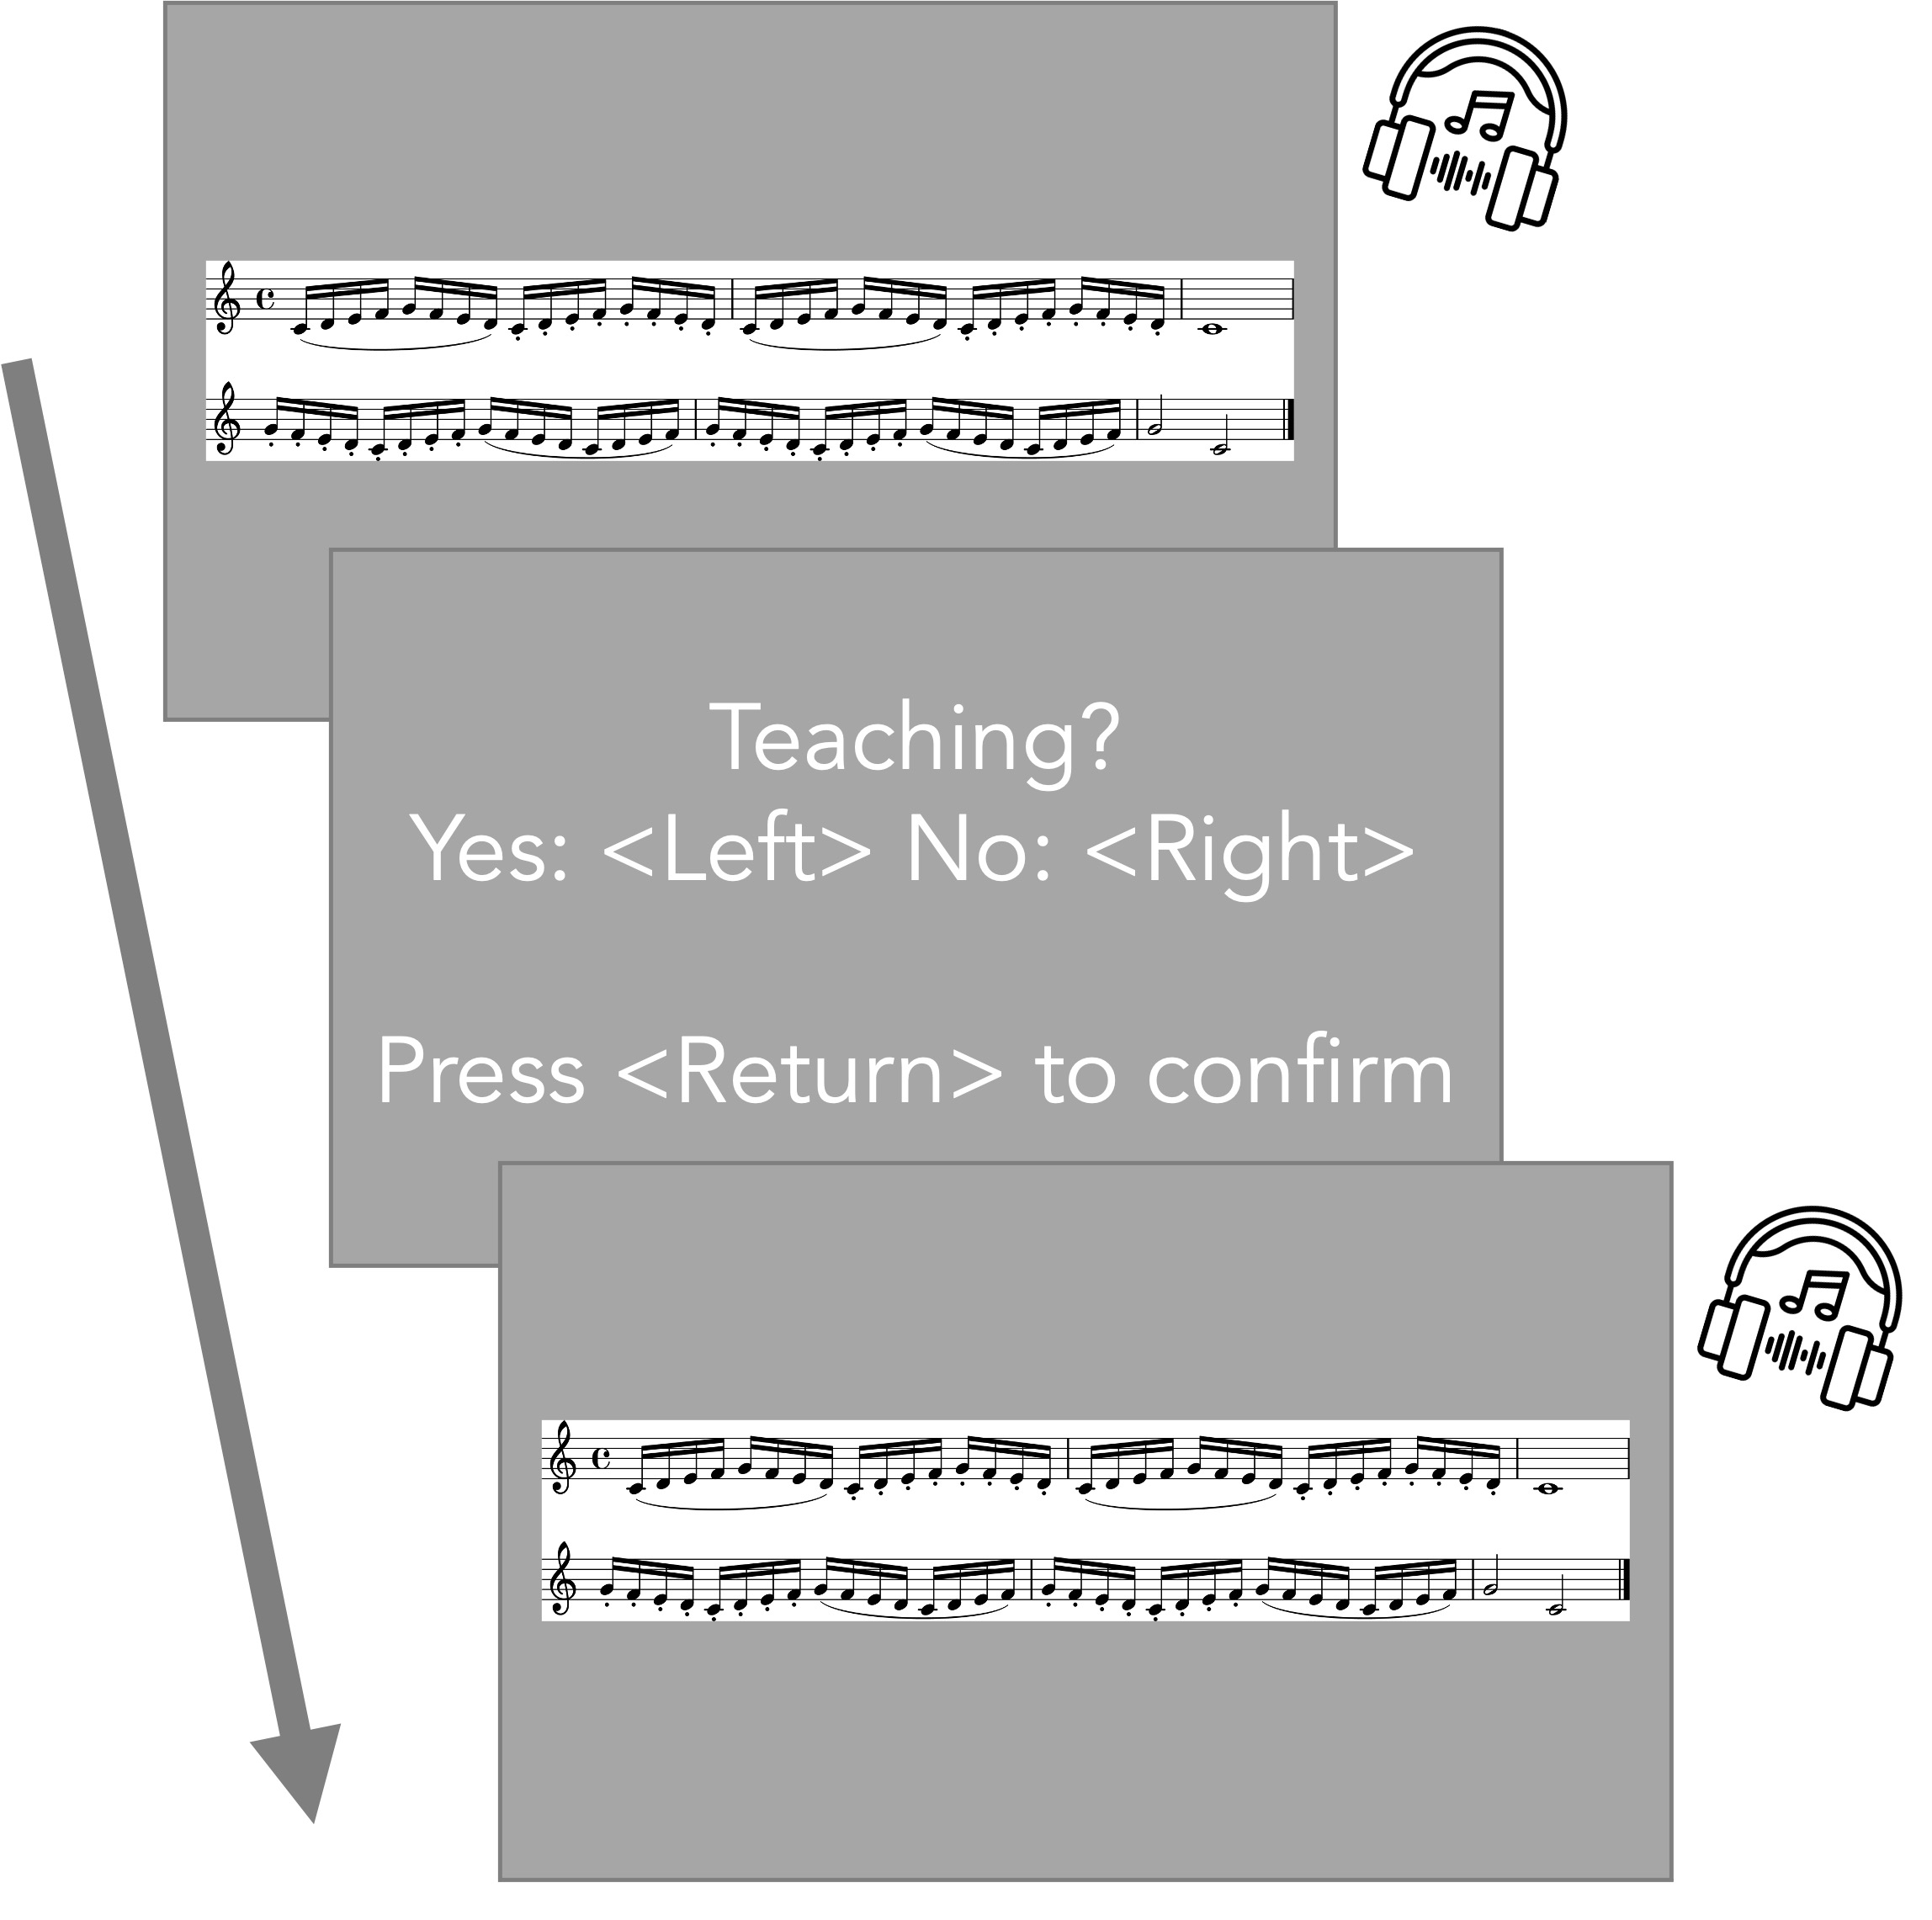
\includegraphics[width=0.5\linewidth]{image/procedure} 

}

\caption{\label{fig:procedure1}Procedure. Participants listened to a recording via headphones while corresponding sheet music was displayed on a monitor. They were required to respond by pressing a left-arrow (yes) or right-arrow (no) key for each judgment. Headphone image from Flaticon.com}\label{fig:procedure-1}
\end{figure}

\clearpage

\hypertarget{results}{%
\section{Results}\label{results}}

All results were reported as significant at \emph{p} \textless{} 0.05.

\hypertarget{accuracy-1}{%
\subsection{Accuracy}\label{accuracy-1}}

A one sample \emph{t}-test was performed to compare the accuracy of participants' judgments against the chance level (50\%). The mean percentage of correct answers {[}\emph{M} = 52.7, \emph{SD} = 4.90{]} was significantly higher than chance (\emph{t}(19) = 2.47, \emph{p} = 0.02, cohen's \emph{d} = 0.55).

We also performed a one sample \emph{t}-test for each technique separately. For articulation, the mean percentage of correct answers {[}\emph{M} = 50.2, \emph{SD} = 6.55{]} was not significantly different from chance (\emph{t}(19) = 0.14, \emph{p} = 0.89, cohen's \emph{d} = 0.03). For dynamics, the mean percentage of correct answers {[}\emph{M} = 55.2, \emph{SD} = 7.81{]} was significantly higher than chance (\emph{t}(19) = 2.98, \emph{p} = 0.01, cohen's \emph{d} = 0.67). A paired \emph{t}-test revealed that there was a significant difference between the two techniques in terms of the accuracy (\emph{t}(19) = -2.12, \emph{p} = 0.05, cohen's \emph{d} = -0.69), suggesting participants chose correct answers more for dynamics recordings than articulation recordings.

\hypertarget{correlation}{%
\subsection{Correlation}\label{correlation}}

\hypertarget{tempo-iois}{%
\subsubsection{Tempo (IOIs)}\label{tempo-iois}}

Performance tempi (IOIs) were significantly correlated with participants' judgments as teaching for both techniques (Articulation; \emph{r(46)} = .77, \emph{p} \textless{} 0.001, Dynamics; \emph{r(46)} = .42, \emph{p} = 0.003, \emph{Figure \ref{fig:ioi-1}}). Participants tended to identify slower performances as teaching.

\hypertarget{articulation-kot}{%
\subsubsection{Articulation (KOT)}\label{articulation-kot}}

For articulation recordings, there was a significant relationship between KOT values and participants' judgments as teaching (\emph{Figure \ref{fig:kot-1}}, left). Specifically, performances with shorter staccato (\emph{r(46)} = -.73, \emph{p} \textless{} 0.001) and longer legato (\emph{r(46)} = .40, \emph{p} = 0.005) were more likely to be judged as teaching.

For dynamics recordings, there was no significant relationship between KOT values and participants' judgments as teaching (Forte; \emph{r(46)} = -.04, \emph{p} = 0.81, Piano; \emph{r(46)} = -.19, \emph{p} = 0.19, \emph{Figure \ref{fig:kot-1}}, right).

\hypertarget{dynamics-kv}{%
\subsubsection{Dynamics (KV)}\label{dynamics-kv}}

For dynamics recordings, there was a significant relationship between KV values and participants' judgments as teaching (\emph{Figure \ref{fig:vel-1}}, right). Specifically, performances with louder forte were more likely to be judged as teaching (\emph{r(46)} = .45, \emph{p} = 0.001). However, there was no significant relationship between KV values for piano and participants' judgments as teaching (\emph{r(46)} = -.22, \emph{p} = 0.13).

For articulation recordings, there was no significant relationship between KV values and participants' judgments as teaching (Legato; \emph{r(46)} = .10, \emph{p} = 0.52, Staccato; \emph{r(46)} = -.02, \emph{p} = 0.87, \emph{Figure \ref{fig:vel-1}}, left).

\hypertarget{dynamics-contrast-kv-diff}{%
\subsubsection{Dynamics contrast (KV-Diff)}\label{dynamics-contrast-kv-diff}}

For dynamics recordings, there was a significant relationship between KV difference between forte and piano and participants' judgments as teaching (\emph{Figure \ref{fig:vel-diff-1}}, right). Specifically, performances with larger contrasts between forte and piano were more likely to be judged as teaching (From Forte to Piano; \emph{r(46)} = -.50, \emph{p} \textless{} 0.001, From Piano to Forte; \emph{r(46)} = .62, \emph{p} \textless{} 0.001).

For articulation recordings, there was no significant relationship between KV difference between legato and staccato and participants' judgments as teaching (From Legato to Staccato; \emph{r(46)} = -.26, \emph{p} = 0.071, From Staccato to Legato; \emph{r(46)} = -.19, \emph{p} = 0.21, \emph{Figure \ref{fig:vel-diff-1}}, left).

\hypertarget{multiple-regression}{%
\subsection{Multiple regression}\label{multiple-regression}}

In order to further explore which feature of performance contributed the most to participants' judgments as teaching, multiple regression analyses were conducted. Statistical model assumptions were tested using the \emph{performance} R package (Lüdecke, Ben-Shachar, Patil, Waggoner, \& Makowski, 2021) and most of the assumptions (see \emph{Supplementary Material} for details) were met. Since articulation and dynamics consisted of two opposite subcomponents (i.e., legato vs.~staccato, forte vs.~piano) and therefore cannot be summed up to represent each technique as one value, we reported four separate regression models for each subcomponent (see details in \emph{Data analysis}).

\hypertarget{legato}{%
\subsubsection{Legato}\label{legato}}

A multiple regression analysis was conducted to predict participants' judgments as teaching based on performance features of tempo (IOIs), articulation (KOT for legato parts), dynamics (KV for legato parts) and dynamics contrast (KV-Diff from legato to staccato). The result of the regression indicated that the model explained 64.6 \% of the variance (\emph{F}(4, 43) = 22.5, \emph{p} \textless{} 0.001). It was found that tempo (IOIs; \emph{\(\beta\)} = 0.78, \emph{p} \textless{} 0.001) and articulation for the legato parts (KOT; \emph{\(\beta\)} = 0.26, \emph{p} = 0.004) were significant predictors of participants' judgments as teaching.

\hypertarget{staccato}{%
\subsubsection{Staccato}\label{staccato}}

A multiple regression analysis was conducted to predict participants' judgments as teaching based on performance features of tempo (IOIs), articulation (KOT for staccato parts), dynamics (KV for staccato parts) and dynamics contrast (KV-Diff from staccato to legato). The result of the regression indicated that the model explained 64.0 \% of the variance (\emph{F}(4, 43) = 21.9, \emph{p} \textless{} 0.001). It was found that tempo (IOIs; \emph{\(\beta\)} = 0.52, \emph{p} = 0.002) and articulation for the staccato parts (KOT; \emph{\(\beta\)} = -0.28, \emph{p} = 0.020) were significant predictors of participants' judgments as teaching.

\hypertarget{forte}{%
\subsubsection{Forte}\label{forte}}

A multiple regression analysis was conducted to predict participants' judgments as teaching based on performance features of tempo (IOIs), articulation (KOT for forte parts), dynamics (KV for forte parts) and dynamics contrast (KV-Diff from forte to piano). The result of the regression indicated that the model explained 35.9 \% of the variance (\emph{F}(4, 43) = 7.58, \emph{p} \textless{} 0.001). It was found that tempo (IOIs; \emph{\(\beta\)} = 0.35, \emph{p} = 0.007) and dynamics for the forte parts (KV; \emph{\(\beta\)} = 0.73, \emph{p} = 0.048) were significant predictors of participants' judgments as teaching.

\hypertarget{piano}{%
\subsubsection{Piano}\label{piano}}

A multiple regression analysis was conducted to predict participants' judgments as teaching based on performance features of tempo (IOIs), articulation (KOT for piano parts), dynamics (KV for piano parts) and dynamics contrast (KV-Diff from piano to forte). The result of the regression indicated that the model explained 51.2 \% of the variance (\emph{F}(4, 43) = 13.3, \emph{p} \textless{} 0.001). It was found that tempo (IOIs; \emph{\(\beta\)} = 0.38, \emph{p} \textless{} 0.001) and dynamics contrast from piano to forte (KV-Diff; \emph{\(\beta\)} = 0.99, \emph{p} \textless{} 0.001) were significant predictors of participants' judgments as teaching.

\begin{figure}

{\centering \includegraphics[width=0.7\linewidth]{manuscript_files/figure-latex/plot-ioi-1-1} 

}

\caption{\label{fig:ioi-1}Experiment 1: Scatter plot showing the correlation between tempo feature (IOIs) and average participants' judgments as teaching for each recording. Therefore, each dot represents each stimulus.}\label{fig:plot-ioi-1}
\end{figure}

\begin{figure}

{\centering \includegraphics[width=0.7\linewidth]{manuscript_files/figure-latex/plot-kot-1-1} 

}

\caption{\label{fig:kot-1}Experiment 1: Scatter plot showing the correlation between articulation feature (KOT) and average participants' judgments as teaching for each recording. Therefore, each dot represents each stimulus.}\label{fig:plot-kot-1}
\end{figure}

\begin{figure}

{\centering \includegraphics[width=0.7\linewidth]{manuscript_files/figure-latex/plot-vel-1-1} 

}

\caption{\label{fig:vel-1}Experiment 1: Scatter plot showing the correlation between dynamics feature (KV) and average participants' judgments as teaching for each recording. Therefore, each dot represents each stimulus.}\label{fig:plot-vel-1}
\end{figure}

\begin{figure}

{\centering \includegraphics[width=0.7\linewidth]{manuscript_files/figure-latex/plot-vel-diff-1-1} 

}

\caption{\label{fig:vel-diff-1}Experiment 1: Scatter plot showing the correlation between dynamics contrast feature (KV-Diff) and average participants' judgments as teaching for each recording. Therefore, each dot represents each stimulus.}\label{fig:plot-vel-diff-1}
\end{figure}

\clearpage

\hypertarget{discussion}{%
\section{Discussion}\label{discussion}}

Experiment 1 investigated whether musicians could distinguish teaching recordings from performing recordings accurately and which features of piano performance made them infer teaching intentions. The results demonstrated that musicians could choose correct answers above chance. Also, it was found that the accuracy of participants' judgments was better for dynamics recordings than for articulation recordings. When it comes to how performance features contributed to participants' judments, performances with slower tempo were more likely to be judged as teaching by musicians regardless of which expressive technique was implemented in the piece. For articulation recordings, performances with longer legato and shorter staccato were tended to be judged as teaching. For dynamics recordings, performances with louder forte were more likely to be judged as teaching whereas there was no relationship between softer sound (i.e., piano) and participants' judgments as teaching. Importantly, performances with larger contrast between forte and piano for both directions (i.e., from forte to piano, from piano to forte) were more likely to be judged as teaching. This result may suggest that dynamics contrast might be reliably used to infer teaching intentions, rather than absolute dynamics values themselves. Moreover, multiple regression analyses implied that tempo feature was the strongest predictor of participants' judgments as teaching in general whereas there were specific predictors depending on which expressive technique was implemented in the piece. These performance features were overall consistent with what expert pianists did in our previous experiments for teaching purposes. Therefore, our findings suggest that musicians may rely on generic pedagogical behaviours (e.g., slower demonstration, exaggeration) to infer teaching intentions of expert pianists, only by listening to recorded performances.

\clearpage

\hypertarget{experiment-2}{%
\section{Experiment 2}\label{experiment-2}}

The aim of Experiment 2 was to replicate the findings in Experiment 1 with a more naturalistic piece of music. Given the findings in Experiment 1, we predicted that slower performance would be likely to be judged as teaching regardless of which expressive technique (articulation or dynamics) was implemented. Also performances with exaggerated articulation and dynamics (in particular, longer legato and shorter staccato, larger contrast between forte and piano) would be likely to be judged as teaching.

\hypertarget{methods-1}{%
\section{Methods}\label{methods-1}}

\hypertarget{participants-1}{%
\subsection{Participants}\label{participants-1}}

We recruited 21 participants who had at least six years of training in any musical instrument or singing. They were able to read sheet music and know two musical expressive techniques of articulation and dynamics. One participant was excluded because s/he did not understand the instructions. Therefore, 20 participants (Female: 10) were included for data analysis and had 12.65 years of training on average in any musical instrument or singing (\emph{SD} = 5.40). Most people were right-handed (Left; 1) with a mean age of 33.55 (\emph{SD} = 12.80). As Experiment 1, all participants were recruited through the SONA system and the study (No.~2020/02) was approved by the PREBO CEU PU in Austria.

\hypertarget{apparatus-and-procedure}{%
\subsection{Apparatus and procedure}\label{apparatus-and-procedure}}

The apparatus and procedure were identical to Experiment 1 except that each block consisted of four practice trials and 36 experimental trials. The number of trials was reduced due to the time constraint of the experiment.

\hypertarget{stimuli-1}{%
\subsection{Stimuli}\label{stimuli-1}}

As Experiment 1, we selected stimuli from our previous experiments (Tominaga et al., \emph{submitted}; Experiment 2). The excerpt was taken from ``Sonatina Op.36 (No.3) in C major'' by Muzio Clementi and modified for the experiment. The excerpt was performed with either articulation (\emph{Figure \ref{fig:stim2}}, A) or dynamics (\emph{Figure \ref{fig:stim2}}, B). The stimuli were performed around 100 - 120 quarter-beats per minute.

For the current experiment, 72 performances were chosen from the valid performances in Tominaga et al.~(\emph{submitted}; Experiment 2). There were 248 valid performances in the teaching condition and 256 valid performances in the performing condition. We randomly sampled 18 articulation performances and 18 dynamics performances from the teaching condition as well as 18 articulation performances and 18 dynamics performances from the performing condition. Again, it is important to note that each performance from the teaching condition did not necessarily exhibit specific features of teaching that we found in the previous experiments (e.g., exaggeration) since we randomly sampled the performances.

\hypertarget{data-analysis-1}{%
\subsection{Data analysis}\label{data-analysis-1}}

The data analysis was almost identical to Experiment 1. Only the 8th notes with expressive notations were included for data analysis. As a result, only one 8th note in the 4th measure without any expression was not included.

\begin{figure}
\includegraphics[width=1\linewidth]{manuscript_files/figure-latex/stim-2-1} \caption{\label{fig:stim2}Stimuli. (A)Articulation. The curved line (slur) indicates legato and the dots indicate staccato. (B)Dynamics. The symbol `f' denotes forte and the symbol `p' denotes piano. Only the 8th notes with expressive notations were used for data analysis.}\label{fig:stim-2}
\end{figure}

\hypertarget{results-1}{%
\section{Results}\label{results-1}}

All results were reported as significant at \emph{p} \textless{} 0.05.

\hypertarget{accuracy-2}{%
\subsection{Accuracy}\label{accuracy-2}}

A one sample \emph{t}-test was performed to compare the accuracy of participants' judgments against the chance level (50\%). The mean percentage of correct answers {[}\emph{M} = 52.8, \emph{SD} = 4.78{]} was significantly higher than chance (\emph{t}(19) = 2.66, \emph{p} = 0.02, cohen's \emph{d} = 0.60).

We also performed a one sample \emph{t}-test for each technique separately. For articulation, the mean percentage of correct answers {[}\emph{M} = 52.4, \emph{SD} = 6.94{]} was not significantly different from chance (\emph{t}(19) = 1.52, \emph{p} = 0.14, cohen's \emph{d} = 0.34). Also for dynamics, the mean percentage of correct answers {[}\emph{M} = 53.3, \emph{SD} = 8.53{]} was not significantly different from chance (\emph{t}(19) = 1.75, \emph{p} = 0.10, cohen's \emph{d} = 0.39). A paired \emph{t}-test revealed that there was no significant difference between the two techniques in terms of the accuracy (\emph{t}(19) = -0.35, \emph{p} = 0.73, cohen's \emph{d} = -0.13).

\hypertarget{correlation-1}{%
\subsection{Correlation}\label{correlation-1}}

\hypertarget{tempo-iois-1}{%
\subsubsection{Tempo (IOIs)}\label{tempo-iois-1}}

Unlike Experiment 1, there was a significant relationship between performance tempi (IOIs) and participants' judgments as teaching only for dynamics recordings (Articulation; \emph{r(34)} = .25, \emph{p} = 0.15, Dynamics; \emph{r(34)} = .39, \emph{p} = 0.02, \emph{Figure \ref{fig:ioi-2}}). Participants tended to identify slower performances as teaching for dynamics recordings.

\hypertarget{articulation-kot-1}{%
\subsubsection{Articulation (KOT)}\label{articulation-kot-1}}

Unlike Experiment 1, for articulation recordings, there was no significant relationship between KOT values and participants' judgments as teaching (Legato; \emph{r(34)} = -.03, \emph{p} = 0.39, Staccato; \emph{r(34)} = -.15, \emph{p} = 0.39, \emph{Figure \ref{fig:kot-2}}, left).

For dynamics recordings, there was no significant relationship between KOT values for forte and participants' judgments as teaching (\emph{r(34)} = -.11, \emph{p} = 0.52). However, there was a significant relationship between KOT values for piano and participants' judgments as teaching (\emph{r(34)} = -.35, \emph{p} = 0.034), suggesting that performances with staccato-style piano were more likely to be considered as teaching performance (\emph{Figure \ref{fig:kot-2}}, right).

\hypertarget{dynamics-kv-1}{%
\subsubsection{Dynamics (KV)}\label{dynamics-kv-1}}

As Experiment 1, for dynamics recordings, there was a significant relationship between KV values and participants' judgments as teaching (\emph{Figure \ref{fig:vel-2}}, right). Specifically, performances with louder forte (\emph{r(34)} = .45, \emph{p} = 0.007) and softer piano (\emph{r(34)} = -.45, \emph{p} = 0.006) were more likely to be judged as teaching.

For articulation recordings, there was no significant relationship between KV values and participants' judgments as teaching (Legato; \emph{r(34)} = .08, \emph{p} = 0.63, Staccato; \emph{r(34)} = .21, \emph{p} = 0.22, \emph{Figure \ref{fig:vel-2}}, left).

\hypertarget{dynamics-contrast-kv-diff-1}{%
\subsubsection{Dynamics contrast (KV-Diff)}\label{dynamics-contrast-kv-diff-1}}

As Experiment 1, for dynamics recordings, there was a significant relationship between KV difference between forte and piano and participants' judgments as teaching (\emph{Figure \ref{fig:vel-diff-2}}, right). Specifically, performances with larger contrasts between forte and piano were more likely to be judged as teaching (From Forte to Piano; \emph{r(34)} = -.75, \emph{p} \textless{} 0.001, From Piano to Forte; \emph{r(34)} = .59, \emph{p} \textless{} 0.001).

For articulation recordings, there was no significant relationship between KV difference between transition points from legato to staccato and participants' judgments as teaching (\emph{r(34)} = .23, \emph{p} = 0.176). However, there was a significant relationship between the transition points from staccato to legato and participants' judgments as teaching (\emph{r(34)} = .36, \emph{p} = 0.03), suggesting that performances with larger contrast from staccato to legato were more likely to be considered as teaching performance (\emph{Figure \ref{fig:vel-diff-2}}, left).

\hypertarget{multiple-regression-1}{%
\subsection{Multiple regression}\label{multiple-regression-1}}

As Experiment 1, we performed multiple regression analyses to further explore which feature of performance contributed the most to participants' judgments as teaching. Statistical model assumptions were tested and most of the assumptions (see \emph{Supplementary Material} for details) were met. Again, since articulation and dynamics consisted of two opposite subcomponents (i.e., legato vs.~staccato, forte vs.~piano) and therefore cannot be summed up to represent each technique as one value, we reported four separate regression models for each subcomponent (see details in \emph{Data analysis} in Experiment 1).

\hypertarget{legato-1}{%
\subsubsection{Legato}\label{legato-1}}

A multiple regression analysis was conducted to predict participants' judgments as teaching based on performance features of tempo (IOIs), articulation (KOT for legato parts), dynamics (KV for legato parts) and dynamics contrast (KV-Diff from legato to staccato). The result of the regression indicated that the model explained 19.8 \% of the variance (\emph{F}(4, 31) = 3.16, \emph{p} = 0.028). It was found that tempo (IOIs; \emph{\(\beta\)} = 0.58, \emph{p} = 0.011), dynamics (KV; \emph{\(\beta\)} = 1.10, \emph{p} = 0.018) and dynamics contrast (KV-Diff; \emph{\(\beta\)} = 1.90, \emph{p} = 0.006) for the legato parts were articulation for the legato parts were significant predictors of participants' judgments as teaching. However, articulation (KOT; \emph{\(\beta\)} = -0.08, \emph{p} = 0.47) for the legato parts was not a significant predictor as opposed to Experiment 1.

\hypertarget{staccato-1}{%
\subsubsection{Staccato}\label{staccato-1}}

A multiple regression analysis was conducted to predict participants' judgments as teaching based on performance features of tempo (IOIs), articulation (KOT for staccato parts), dynamics (KV for staccato parts) and dynamics contrast (KV-Diff from staccato to legato). The overall model was not statistically significant (\(R^{2}\) = 12.3, \emph{F}(4, 31) = 2.22, \emph{p} = 0.09).

\hypertarget{forte-1}{%
\subsubsection{Forte}\label{forte-1}}

A multiple regression analysis was conducted to predict participants' judgments as teaching based on performance features of tempo (IOIs), articulation (KOT for forte parts), dynamics (KV for forte parts) and dynamics contrast (KV-Diff from forte to piano). The result of the regression indicated that the model explained 60.7 \% of the variance (\emph{F}(4, 31) = 14.5, \emph{p} \textless{} 0.001). It was found that dynamics contrast from forte to piano (KV-Diff; \emph{\(\beta\)} = -1.64, \emph{p} \textless{} 0.001) were significant predictors of participants' judgments as teaching.

\hypertarget{piano-1}{%
\subsubsection{Piano}\label{piano-1}}

A multiple regression analysis was conducted to predict participants' judgments as teaching based on performance features of tempo (IOIs), articulation (KOT for piano parts), dynamics (KV for piano parts) and dynamics contrast (KV-Diff from piano to forte). The result of the regression indicated that the model explained 49.5 \% of the variance (\emph{F}(4, 31) = 9.57, \emph{p} \textless{} 0.001). It was found that tempo (IOIs; \emph{\(\beta\)} = 0.55, \emph{p} = 0.022) and dynamics contrast from piano to forte (KV-Diff; \emph{\(\beta\)} = 1.09, \emph{p} \textless{} 0.001) were significant predictors of participants' judgments as teaching.

\begin{figure}

{\centering \includegraphics[width=0.7\linewidth]{manuscript_files/figure-latex/plot-ioi-2-1} 

}

\caption{\label{fig:ioi-2}Experiment 2: Scatter plot showing the correlation between tempo featurea (IOIs) and average participants' judgments as teaching for each recording. Therefore, each dot represents each stimulus.}\label{fig:plot-ioi-2}
\end{figure}

\begin{figure}

{\centering \includegraphics[width=0.7\linewidth]{manuscript_files/figure-latex/plot-kot-2-1} 

}

\caption{\label{fig:kot-2}Experiment 2: Scatter plot showing the correlation between articulation features (KOT) and average participants' judgments as teaching for each recording. Therefore, each dot represents each stimulus.}\label{fig:plot-kot-2}
\end{figure}

\begin{figure}

{\centering \includegraphics[width=0.7\linewidth]{manuscript_files/figure-latex/plot-vel-2-1} 

}

\caption{\label{fig:vel-2}Experiment 2: Scatter plot showing the correlation between dynamics features (KV) and average participants' judgments as teaching for each recording. Therefore, each dot represents each stimulus.}\label{fig:plot-vel-2}
\end{figure}

\begin{figure}

{\centering \includegraphics[width=0.7\linewidth]{manuscript_files/figure-latex/plot-vel-diff-2-1} 

}

\caption{\label{fig:vel-diff-2}Experiment 2: Scatter plot showing the correlation between dynamics contrast features (KV-Diff) and average participants' judgment as teaching for each stimulus.}\label{fig:plot-vel-diff-2}
\end{figure}

\hypertarget{discussion-1}{%
\section{Discussion}\label{discussion-1}}

The aim of Experiment 2 was to replicate the results of Experiment 1 with a more naturalistic piece of music. However, unlike Experiment 1, tempo (IOIs) does not seem to contribute to participants' judgments as teaching. This could be that in a musically complex piece, tempo might have been considered to be one of the interpretations of music and was not used as a reliable cue to infer teaching intentions. Also, articulation (KOT) does not seem to contribute to participants' judgments as teaching. As Experiment 1, dynamics (KV) seems to be used as a reliable cue to detect the characteristic of teaching performance. We could successfully replicate that performances with larger contrast between forte and piano seem to be considered as teaching. Moreover, performances with both exaggerated forte and piano were considered to be for teaching. These consistent results suggest that loudness (dynamics) might be used as a reliable cue to infer teaching intentions regardless of the complexity of a musical piece.

Multiple regression analyses also implied that tempo feature was not a strong predictor of participants' judgments as teaching when listening to a musically complex piece. However, dynamics contrast seems to be a strong predictor of participants' judgments as teaching, especially for dynamics recordings. This finding also suggests that loudness might be a strong cue to infer pedagogical intentions even in a naturalistic piece of music.

\hypertarget{general-discussion}{%
\section{General discussion}\label{general-discussion}}

The present study investigated whether and how musician infer pedagogical intentions by listening to piano recordings. In both Experiment 1 and 2, participants were able to choose correct answers accurately more than chance (50\%). However, the results showed that the accuracy was relatively low (52.7 \% in Experiment 1; 52.8 \% in Experiment 2). This might be because the stimuli were randomly sampled from the teaching and performing condition in Tominaga et al.~(\emph{submitted}) and all the selected recordings did not exhibit the characteristics of teaching performance (e.g., slow performance, exaggeration). The reason why we randomly selected the stimuli from each condition (i.e., teaching or performing) was because all the characteristics of teaching performance (e.g., IOIs, KOT, KV) were intercorrelated and it was difficult to choose stimuli based on one single criterion. Future research should examine if musicians answer more accurately with more experimentally controlled stimuli.

In order to examine which features of piano performance make musicians infer pedagogical intentions, we performed correlation and multiple regression analysis. Across the two experiments, it was found that loudness, particularly larger contrast between forte and piano, strongly contributed to participants' judgments when listening to dynamics recordings. On the other hand, unlike what we predicted, slower performance was only considered to be for teaching in Experiment 1 where the stimuli consisted of a simple musical scale. Also, we could not find that performances with exaggerated articulation (e.g., longer legato and shorter staccato) were more likely to be judged as teaching in Experiment 2. This might suggest that some characteristics of performance are not necessarily used or reliable to infer performers' intentions when listening to musically complex pieces. It can be speculated that certain modulations are too subtle so that participants could not perceive them. Another possibility is that modulations can also be considered as one of the expressions or interpretations.

In the current study, we exclusively recruited musicians to explore our research questions. The reason why we recruited musicians only was because the concepts of articulation and dynamics seem to be difficult for those who don't play an instrument to understand in the current settings. It would be important to investigate how novices perceive and infer pedagogical intentions differently from musicians, who already have some experience in playing music.

\newpage

\hypertarget{references}{%
\section{References}\label{references}}

\begingroup
\setlength{\parindent}{-0in}
\setlength{\leftskip}{0in}

\hypertarget{refs}{}
\begin{CSLReferences}{1}{0}
\leavevmode\vadjust pre{\hypertarget{ref-akkermans_2019}{}}%
Akkermans, J., Schapiro, R., Müllensiefen, D., Jakubowski, K., Shanahan, D., Baker, D., \ldots{} Frieler, K. (2019). Decoding emotions in expressive music performances: {A} multi-lab replication and extension study. \emph{Cognition and Emotion}, \emph{33}(6), 1099--1118. \url{https://doi.org/10.1080/02699931.2018.1541312}

\leavevmode\vadjust pre{\hypertarget{ref-brand_2002}{}}%
Brand, R. J., Baldwin, D. A., \& Ashburn, L. A. (2002). Evidence for {``motionese''}: Modifications in mothers' infant-directed action. \emph{Developmental Science}, \emph{5}(1), 72--83. \url{https://doi.org/10.1111/1467-7687.00211}

\leavevmode\vadjust pre{\hypertarget{ref-bresin_2000}{}}%
Bresin, R., \& Battel, G. U. (2000). Articulation {Strategies} in {Expressive Piano Performance Analysis} of {Legato}, {Staccato}, and {Repeated Notes} in {Performances} of the {Andante Movement} of {Mozart}'s {Sonata} in {G Major} ({K} 545). \emph{Journal of New Music Research}, \emph{29}(3), 211--224. \url{https://doi.org/10.1076/jnmr.29.3.211.3092}

\leavevmode\vadjust pre{\hypertarget{ref-csibra_2009}{}}%
Csibra, G., \& Gergely, G. (2009). Natural pedagogy. \emph{Trends in Cognitive Sciences}, \emph{13}(4), 148--153. \url{https://doi.org/10.1016/j.tics.2009.01.005}

\leavevmode\vadjust pre{\hypertarget{ref-gabrielsson_1996}{}}%
Gabrielsson, A., \& Juslin, P. N. (1996). Emotional {Expression} in {Music Performance}: {Between} the {Performer}'s {Intention} and the {Listener}'s {Experience}. \emph{Psychology of Music}, \emph{24}(1), 68--91. \url{https://doi.org/10.1177/0305735696241007}

\leavevmode\vadjust pre{\hypertarget{ref-gweon_2020}{}}%
Gweon, H. (2020). The role of communication in acquisition, curation, and transmission of culture. \emph{Behavioral and Brain Sciences}, \emph{43}. \url{https://doi.org/10.1017/S0140525X19002863}

\leavevmode\vadjust pre{\hypertarget{ref-ludecke_2021}{}}%
Lüdecke, D., Ben-Shachar, M. S., Patil, I., Waggoner, P., \& Makowski, D. (2021). Performance: {An R Package} for {Assessment}, {Comparison} and {Testing} of {Statistical Models}. \emph{Journal of Open Source Software}, \emph{6}(60), 3139. \url{https://doi.org/10.21105/joss.03139}

\leavevmode\vadjust pre{\hypertarget{ref-mcellin_2017}{}}%
McEllin, L., Knoblich, G., \& Sebanz, N. (2017). Distinct kinematic markers of demonstration and joint action coordination? {Evidence} from virtual xylophone playing. \emph{Journal of Experimental Psychology: Human Perception and Performance}, \emph{44}(6), 885. \url{https://doi.org/10.1037/xhp0000505}

\leavevmode\vadjust pre{\hypertarget{ref-mcellin_2018}{}}%
McEllin, L., Sebanz, N., \& Knoblich, G. (2018). Identifying others' informative intentions from movement kinematics. \emph{Cognition}, \emph{180}, 246--258. \url{https://doi.org/10.1016/j.cognition.2018.08.001}

\leavevmode\vadjust pre{\hypertarget{ref-saint-georges_2013}{}}%
Saint-Georges, C., Chetouani, M., Cassel, R., Apicella, F., Mahdhaoui, A., Muratori, F., \ldots{} Cohen, D. (2013). Motherese in {Interaction}: {At} the {Cross-Road} of {Emotion} and {Cognition}? ({A Systematic Review}). \emph{PLOS ONE}, \emph{8}(10), e78103. \url{https://doi.org/10.1371/journal.pone.0078103}

\leavevmode\vadjust pre{\hypertarget{ref-tennie_2009}{}}%
Tennie, C., Call, J., \& Tomasello, M. (2009). Ratcheting up the ratchet: On the evolution of cumulative culture. \emph{Philosophical Transactions of the Royal Society B: Biological Sciences}, \emph{364}(1528), 2405--2415. \url{https://doi.org/10.1098/rstb.2009.0052}

\leavevmode\vadjust pre{\hypertarget{ref-tomasello_1993}{}}%
Tomasello, M., Kruger, A. C., \& Ratner, H. H. (1993). Cultural learning. \emph{Behavioral and Brain Sciences}, \emph{16}(3), 495--511. \url{https://doi.org/10.1017/S0140525X0003123X}

\leavevmode\vadjust pre{\hypertarget{ref-uther_2007}{}}%
Uther, M., Knoll, M. A., \& Burnham, D. (2007). Do you speak {E-NG-L-I-SH}? {A} comparison of foreigner- and infant-directed speech. \emph{Speech Communication}, \emph{49}(1), 2--7. \url{https://doi.org/10.1016/j.specom.2006.10.003}

\leavevmode\vadjust pre{\hypertarget{ref-veissiere_2020}{}}%
Veissière, S. P. L., Constant, A., Ramstead, M. J. D., Friston, K. J., \& Kirmayer, L. J. (2020). Thinking through other minds: {A} variational approach to cognition and culture. \emph{Behavioral and Brain Sciences}, \emph{43}. \url{https://doi.org/10.1017/S0140525X19001213}

\end{CSLReferences}

\endgroup

\hypertarget{supplementary-materials}{%
\section{Supplementary Materials}\label{supplementary-materials}}

All data is available at .

\hypertarget{acknowledgement}{%
\section{Acknowledgement}\label{acknowledgement}}

This research was supported by the European Research Council under the European Union's Seventh Framework Program (FP7/2007--2013)/ERC Grant agreement no. 609819, SOMICS, and by ERC Grant agreement no. 616072, JAXPERTISE. We thank Fanni Takátsy for her help with data collection.


\end{document}
